% \documentclass[9pt, twoside, openright, showtrimson]{memoir}
\documentclass[10pt, a4paper, twoside, openright]{memoir}

\setstocksize{11in}{8in}
\settrimmedsize{9in}{7in}{*}
\settrims{1in}{.75in}
\settypeblocksize{7.5in}{6in}{*}
\setlrmargins{.85in}{*}{*}
\setulmargins{.5in}{*}{*}
\setheadfoot{\onelineskip}{2\onelineskip}
\setheaderspaces{*}{2\onelineskip}{*}

\checkandfixthelayout

\makeatletter
\DeclareOldFontCommand{\rm}{\normalfont\rmfamily}{\mathrm}
\DeclareOldFontCommand{\sf}{\normalfont\sffamily}{\mathsf}
\DeclareOldFontCommand{\tt}{\normalfont\ttfamily}{\mathtt}
\DeclareOldFontCommand{\bf}{\normalfont\bfseries}{\mathbf}
\DeclareOldFontCommand{\it}{\normalfont\itshape}{\mathit}
\DeclareOldFontCommand{\sl}{\normalfont\slshape}{\@nomath\sl}
\DeclareOldFontCommand{\sc}{\normalfont\scshape}{\@nomath\sc}
\makeatother

% \usepackage{xcolor, calc, graphicx, soul, fourier, verbments, makeidx, mflogo}
\usepackage{xcolor, calc, graphicx, soul, minted, makeidx, mflogo, 
  pstricks, minitoc, amsmath, amssymb, pst-poly}
\let\footruleskip\undefined
\usepackage{fancyhdr}
\pagestyle{fancy}
\usepackage[shellescape, latex]{gmp}
\showtrimson

\definecolor{webred}{rgb}{.7,0,0}
\definecolor{webbg}{rgb}{1,.8,.2}
\usepackage[colorlinks]{hyperref}
\hypersetup{%
  pdftitle={C Programming with C99},
  pdfauthor={Shiv S. Dayal},
  pdfkeywords={C, Programming},
  bookmarksnumbered,
  pdfstartview={FitH},
  urlcolor=webred,
  linkcolor=webred,
}%

\renewcommand{\chaptermark}[1]{%
  \markboth{#1}{}}
\renewcommand{\sectionmark}[1]{%
  \markright{#1}{}}

\definecolor{nicered}{rgb}{.347,.129,.149}
\definecolor{nicegreen}{rgb}{.129,.447,.149}
\definecolor{niceblack}{rgb}{.2, .2, .2}
\definecolor{niceblue}{rgb}{0, 0, .6}
\definecolor{niceyellow}{rgb}{1,1,.95}

%\color{niceblack}
\pagecolor{niceyellow}
\makeatletter
\newlength\dlf@normtxtw
\setlength\dlf@normtxtw{\textwidth}
\def\myhelvetfont{\def\sfdefault{mdput}}
\newsavebox{\feline@chapter}
\newcommand\feline@chapter@marker[1][4cm]{%
  \sbox\feline@chapter{%
    \resizebox{!}{#1}{\fboxsep=1pt%
      \colorbox{niceblack}{\color{white}\bfseries\sffamily\thechapter}%
    }}%
  \rotatebox{90}{%
    \resizebox{%
      \heightof{\usebox{\feline@chapter}}+\depthof{\usebox{\feline@chapter}}}%
    {!}{\scshape\so\@chapapp}}\quad%
  \raisebox{\depthof{\usebox{\feline@chapter}}}{\usebox{\feline@chapter}}%
}
\newcommand\feline@chm[1][4cm]{%
  \sbox\feline@chapter{\feline@chapter@marker[#1]}%
  \makebox[0pt][l]{% aka \rlap
    \makebox[1cm][r]{\usebox\feline@chapter}%
  }}
\makechapterstyle{daleif1}{
  \renewcommand\chapnamefont{\normalfont\Large\scshape\raggedleft\so}
  \renewcommand\chaptitlefont{\normalfont\huge\bfseries\scshape\color{niceblack}}
  \renewcommand\chapternamenum{}
  \renewcommand\printchaptername{}
  \renewcommand\printchapternum{\null\hspace*{5.5in}\feline@chm[1cm]\par}
  \renewcommand\afterchapternum{\par\vskip\midchapskip}
  \renewcommand\printchaptertitle[1]{\chaptitlefont\raggedleft ##1\par}
}
\makeatother
\chapterstyle{daleif1}



\title{\HUGE{\textbf{Computer Programming with 
      GNU/Linux}}\\\vspace*{1cm}\Large{Vol. I}\\\vspace*{1cm}\HUGE{\textbf{C 
      Programming with C99}}\vspace*{2cm}}
\author{\vspace*{1cm}\LARGE{Shiv S. Dayal}}
\date{}

\renewcommand{\ttdefault}{cmtt}
\renewcommand{\contentsname}{Table of Contents}
\makeindex
\begin{document}
\dominitoc
\dominilof
\dominilot
\maketitle
\thispagestyle{empty}
\pagestyle{empty}
\vfill
\newpage
\vspace*{7in}
Copyright, \copyright~ Shiv Shankar Dayal, 2011. All rights reserved.
\newpage
\vspace*{2in}
\begin{center}
  Dedicated to my family\\and Free Software Community
\end{center}
\newpage
\setcounter{page}{1}
\pagenumbering{roman}
\tableofcontents
\newpage
\listoffigures
\newpage
\listoftables
% \newpage
% \listofpyglistings
\newpage
\pagestyle{fancy}
\frontmatter
\setcounter{page}{1} 
\pagenumbering{roman}
\chapter{Preface}
I welcome you to this pdf version of 
\url{https://10hash.com/books/c/} which is a complete rewrite. That 
was my first attempt to write at such a large scale and therefore there were 
many deficiencies in that version which I hope have been countered and
corrected in this version. In the HTML version I had put a lot of emphasis on 
specification. However, the feedback which I got from some of my readers is 
that it has become complicated and is not suitable for beginners. After 
thinking over it I found that it is the order of chpaters which needs to be 
corrected and a lot more examples and exercises need to be there.

In this rewrite I will arrange the chapters in a different way. The empahsis on 
specification will be treated in the last part of book.

\section*{What this book contains?}
This book is about C programming language. In this book I have explained the
syntax of C programming language. But it is not only for learning about
language but how to learn to program using C programming language is also
there. In this book we will follow latest ISO specification of C which is
popularly known as C11.

\section*{Who should read this book?}
People interested in learning C should read this. Anybody can read this book
who has little background on Mathematics. I would say high school education is
sufficient for reading it. So this book is for both beginners and experts
alike. For experts advanced concepts have been presented and also a reference
to standard library has been given along with its usage.

\section*{How to read this book?}
Well, learning programming is like learning a new language and then solving
problems is like Mathematics. So the latter is more important as unless you can
solve the problem on pen and paper, you cannot solve the problems using
C. However, the focus of this book is to explain the features and syntax of C
programming language not on how to solve the problem. To get a good grasp
on the contents of the book one should read the theory first then look at the
examples given and try to understand and run them and in the end attempt
the problems. If you cannot solve the problems then lookup the solution and
try to understand. In case of any problem please log on to my personal
question/answer website \url{http://kunjika.libreprogramming.org/} to get
more help.

\section*{Acknowledgements}
I am in great debt of my family and free software community because both of
these groups have been integral part of my life. Family has prvided direct
support while free software community has provided the freedom and freed me
from the slavery which comes as a package with commercial software. I am
especially grateful to my wife, son and parents because it is their time which
I have borrowed to put in the book. To pay my thanks from free software
community  I will take one name and that is Richard Stallman who started all
this  and is still fighting this never-ending war. When I was doing the Algebra
book then I realized how difficult it is to put Math on web in HTML format and
why Donald Knuth wrote \TeX{}. Also, \TeX{} was one of the first softwares to
be released as a free software. HTML has not yet matured to represent
mathematical content. MathML is supported by Mozilla. Webskit browsers started
supporting  then dropped and I would refrain to comment on commercial browser's support which do not even comply to starndard because they think they are the standards tehmselves and others will bend to their will.

Now as this book is being written using \LaTeX{}~ so obviously Leslie Lamport
and all the people involved with it have my thanks along with Donald Knuth. I
use Emacs with Auctex and hope that someday I will use it in a much more
productive way someday.

I have used TikZ as a tool for drawing all the diagrams. It is a wonderful
package and works very nicely. I have great appreciation for its author Till
Tantau.

%For syntax highlighting I have used \texttt{Verbatim} \LaTeX{} package which
%uses \texttt{pygments} as its backend. You can modify it and make it look
%different both at \LaTeX{} and \texttt{pygments} level. Thanks to the
%respective package authors.

For errors and suggestion please email me at
\href{mailto:shivshankar.dayal@gmail.com}{shivshankar.dayal@gmail.com} where I
will try to respond to each mail as
much as possible. Please use your real names in email not something like
coolguy. As an alternative you can report it at
\url{https://10hash.com} where a question/answer website is maintained.
\begin{flushright}
Shiv Shankar Dayal\\
Nalanda,\\
India, 2015
\end{flushright}

\newpage
\mainmatter
\pagenumbering{arabic}
\chapter{Introduction}
C programming language is a relatively low-level programming language with an
inclination towards system programming. This book will try to serve both as a
tutorial and reference of C programming language. If you have not programmed
earlier then you should read in linear manner. Even if you have programmed it
would be better if you read the book in linear fashion because there are
certain points which you may miss if you skip chapters. Of all popular
mainstream languages C, and Lisp are two oldest but we cannot really say that
Lisp is really popular. It has a niche area(artificial intelligence) and it is
there for that. So let me redefine my statement. Of all general-purpose and
popular programming language C is the oldest. FORTRAN is another very old
language but it is not general purpose programming language. So what makes C so
special that it is still out there. Well, C and Unix were born almost together
in early 1970s. Then Unix was ported in C and the notion that operating systems
can be only written in assembly language, because it has to do time critical
things, was destroyed. After that Unix became very popular. Then when C++ was
not yet there Windows was written in C and more and more programs were written
in C. It might have been the case that Microsoft and Apple would have written
their OS in C++ had it been there. So, essentially what happened that there is
a lot of code base which is there in C. Also, C++'s backward compatibility is
one of the reasons why C++ is so popular. When C was invented there was no
structured programming language and code was mostly written in assembly. With C
it gave the power of assembly and benefits of structured language like code
reuse, modularity, and portability among others. Because of these reasons C
became immensely popular and is still popular. 

C is simple, small, succinct. It may be dirty but is quick. It may have its
quirks but it is a success. C is really so simple yet so deceptive. It will
take one years of programming to really thoroughly understand it.

C is currently described by ISO\/IEC 9899:2011 which you can buy on web or you
can get the draft revision
\url{http://www.open-std.org/jtc1/sc22/wg14/www/docs/n1570.pdf}. It
is not necessary to buy the specification as draft is very much similar. I will
refer to specification in the form of (§ iso.x.x.x.x) to point to sections
where exact information is discussed. Note that specification is written for
accuracy and the language is not trivial to understand. At the same time, it
does not directly address programmers but compiler writers because there are
certain decisions which specification does not make but rather leaves for
compiler authors' decision.

\section{Why C?}
Because it is the most common denominator. Any language be it C++, Java, Perl,
Python etc have got bindings in C. Whenever you are willing to extend these
languages you need to know C. Also, if by any chance you are going towards
system programming you need to C. C is everywhere. There is no escape from
learning it; it does not matter whether you like it or not. 

There is one more important point worth noting here is that C++ is far more
complex compared to C. It is generally accepted that one should not try to
learn C++ as one's first programming language. If you search web then you will
find that many great computer scientists like Ken Thompson, Richard Stallman,
Donald Knuth etc. clearly say that they do not like C++ because it is overly
complex. Also, the runtime(virtual functions) calculations of C++ make it
slightly slower than C. However, C++ has its own strengths and it excels as
well if used properly. Wherever there is a memory constraint or extreme high
performance is needed C is preferred. The simple syntax of C means its code is
very verbose for programmer in the sense that if you read code then you can
very easily see what instructions the code is going to translate into. 

It is very easy to write interfaces to other languages because other languages
expose there objects in terms of C structures not the other way around. The
reason for this is huge popularity of C, maturity and large code base. 

One more important feature is portability. Note that if you want your program
to have high degree of portability then you should not use C99 features but
rather ANSI C because ANSI C compilers are available on most platforms. Even
though Java claims to be portable or other interpreted languages they are
limited by the fact that the interpreters or VMs(JVM in case of Java) is not
available on all the platforms. Therefore, C is the MOST portable language.

One of the advantages with C is that since it is very old a lot of software has
been written using it. GNU/Linux for example uses C for its kernel. GNOME which
is one of the desktop environments of GNU/Linux is also written in C. The fact
is that since a lot of libraries are available in C thus it makes a lot of work
very easy to do in C since the infrastructure or ecosystem is developed and
mature. At the same time, since C is taught in many colleges and universities
as first course in programming a lot of people know C thus if you are writing
free(as in freedom) software then you have a much higher chance of getting
support if you write your code in C.

\section{History}
C was formally delivered to this world in 1972 and conceived by Dennis
MacAlistair Ritchie in 1968. What happened was there was a project for
development of a text processor and GE-645 was bought by AT\&T Bell Labs. At
that time Ken Thompson had developed a game called ``Space Travel''. Then they
had another machine PDP-11. Before that they had PDP-7. Now all the time the
code for ``Space Travel'' had to be rewritten and also the Unix had to be
ported. So when C was invented it was used to write Unix code in C. And then
``Space Travel''. I do not know what was the real motivation the language, the
OS or the game. But such is the story. Also, I have not studied much in this 
about the exact events. In 1972 C was formally announced. C takes its features
from BCPL a language by Martin Richard and B by Ken Thompson. AT\&T Bells labs
gave Unix and a C compiler to many universities at a normal fees and it grew
with leaps and bounds from there and became a ubiquitous language. For many
years ``The C Programming Language'' served as a reference of C. Later it was
standardized by ANSI and then by ISO standards. A very detailed history of C
programming language can be found at
\url{http://cm.bell-labs.com/cm/cs/who/dmr/chist.html} which has been described
by Dennis Ritchie himself.
\index{Dennis Ritchie}
\index{Ken Thompson}

\section{Comparison with Other Languages}
C is a structured, statically typed, somewhat low-level, high-performance
compiled language. It does not support object-oriented programming like most
modern programming including C++, Java, Perl, Python, Ruby etc. However, that
does not mean you cannot do object-oriented programming in C. It is just that C
does not have support at the language level and it is painful to do so. C is
low level because it allows you to handle memory contents directly. You have
something called void which is raw representation of memory content. C also
does not support functional or generic programming but again it is possible to
do so with painful hacks. One of the coveted features is C programs deliver
very high performance if written correctly as it does not have runtime
penalties of virtual functions of OOP (object-oriented programming) languages.

\section{How to learn programming?}
Programming is exactly like Mathematics. As in Mathematics you need to read
theory, understand solved problems and then solve more and more problems by
yourself. If you cannot solve ask your teacher. Similarly, in programming you
need to read about language, try examples given, read code written by others
and then develop your own code. If you get stuck there are umpteen number of
tutorials, mailing lists and groups to help you. I recommend comp.lang.c user
group for C programming. Its interface is at
\url{http://groups.google.com/group/comp.lang.c/}. You should join it and
participate there. \url{http://www.stackoverflow.com/} is also a very good
forum to ask questions about programming in general. You can also come at my
website 
\url{http://kunjika.libreprogramming.org} and ask questions or have a
discussion. 

\section{What is a computer Program?}
Since this book is written for even beginner please allow me to start from
beginning. As the reader may know a computer consists of many components and
one of the most or rather most important part is processor often named as CPU
(central processing unit). The logic gates in CPUs are formed and instructions
like ADD (addition), SUB (subtraction), MUL (multiplication), DIV (division)
etc are implemented in hardware of CPU. When we write a program say C program
the instructions given in our program is translated to a format which operating
system can understand. In our case that is GNU/Linux this executable format is
known as ELF (executable and linkable format). For the curious you can read
\url{http://en.wikipedia.org/wiki/Executable\_and\_Linkable\_Format} and there are
lots of specification for different CPUs. Then operating system interprets
these files and ask CPU to perform action. So a C program does not directly
talk to processor but it rather talks to operating system or kernel of the
operating system and in turn the operating system or kernel provides services
to your program. There is a typical life cycle in development of a C
program. First you, the programmer, uses a text editor like \texttt{Emacs} to
enter the program then you use a compiler like \texttt{gcc} to compile the
program. Then you may get warnings and errors either from prepreocessor,
compiler or linker all of which are wrapped by \texttt{gcc} in one step. Now
there can be error in your compilation command, which, you used to compile the
program or the program itself. If the error is in command then we need to fix
the command or if the error is in program then we need to fix the program and
compile it again. However, only successful compilation does not guarantee that
program is working. It must run well also. If it does not run well then
somewhere in code things are wrong and then we need to either examine the
source code or debug it using a debugger like \texttt{gdb}. Given below is the
complete cycle of what we do in development of a program as a diagram for quick
understanding.

\begin{figure}[t!]
\begin{center}
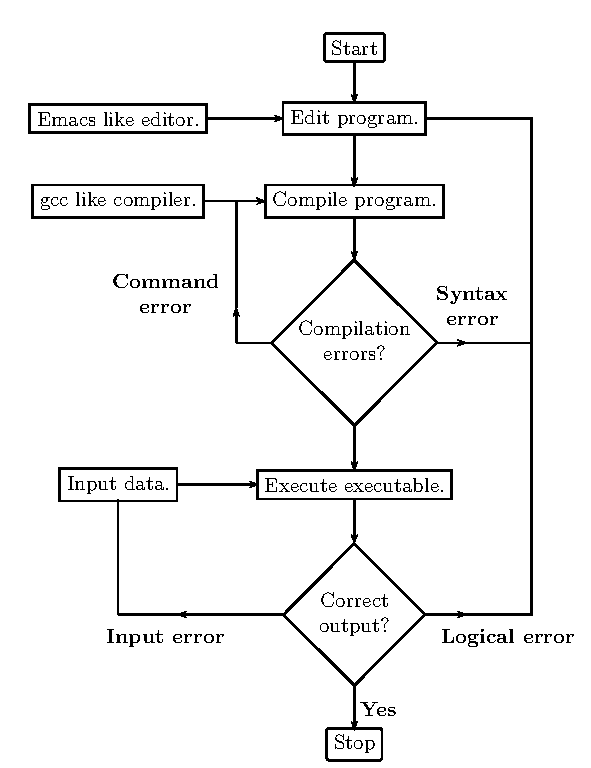
\includegraphics{figs/flowchart-fig1.pdf}
\end{center}
\caption{Life cycle of development of a program}
\end{figure}

\section{Attributes of a Program}
You may be wondering so that is very easy. You just learn programming in C and
start hacking on keyboard to produce software. Well, that is partially true but
a program has several desired attributes which you must consider. Any program
cannot be considered a good program unless it satisfies following requirements
or possess following attributes (Note: These are generic attributes and not
specific to C programming language):
\index{program!attributes}
\begin{enumerate}
\item \textbf{Correctness:}  Correctness means that a program satisfies its
  requirement specification. It means that for a specified input the specified
  output should be produced. This particular attribute is of most
  significance. It does not matter whether other attributes are present or not
  but this one is a must. If a program behavior is not correct then it is of no
  use.
\item \textbf{Efficiency:} Efficiency is second to correctness only. Say you
  are developing a text editor and you take 5 seconds to load a 10KB text file
  then by no means you can persuade a user to use you text editor. A
  program/software must be as efficient as possible. Sometimes it clashes with
  other attributes and also depend on the problem domain that how strict are
  the requirements.
\item \textbf{Security:} A very highly desirable feature in programs which deal
  with more than one computer and also for desktop applications. It is very bad
  if someone can take advantage of buffer overflow, stack overflow, integer
  overflow etc. in your program and you must guard against these at all
  times. Note that to provide security you must put extra checks which will go
  against efficiency.
\item \textbf{Robustness:} Sometimes users will not give correct inputs. For
  example they may enter a character when an integer is asked for or they can
  give input beyond range. In such cases you must handle the erroneous
  input. This is just one example. Sometimes your memory allocation may
  fail. The rule is program defensively. All such input validations and checks
  on memory do take a toll on our second attribute but that does not mean that
  we can neglect it.
\item \textbf{Maintainaibility:} Even a one line program has to be maintained
  if it is worth it! Typically the life of a program far exceeds the
  development time. In almost all the cases the original programmer is not
  maintainer. Because of these reasons you must strive for maintainability. You
  should follow some coding standards like I highly recommend
  \url{http://www.gnu.org/prep/standards/}. Clear documentation is one of the
  prerequisites of maintainability.
\item \textbf{Extensibility:} Let us take our example of text editor and say
  our editor is complete. Now someone else would like to provide a plugin which
  will enable syntax highlighting and project management for this editor. So,
  in order to do so you can choose a plugin-based extensible architecture or
  you can allow them to extend the editor using scripting languages like Guile,
  Python, Lua etc.This features allows user to collaborate and make your
  program better. Remember the rule is the more the merrier here.
\item \textbf{Portability:} It is an elusive and painful but a goal which all
  software desire. Let us say we write our text editor GUI using something like
  Xlib directly then we will have to port the entire GUI for other non X-based
  OSes. So we can choose some cross-platform GUI libraries like GTK+, Qt,
  WxWidgets etc. Even then when system calls come in your software you can do
  not much but either write wrappers and do conditional compilation.
\end{enumerate}

\section{Tools of the Trade}
At the very least you need a compiler, an editor and a linker. Almost all
GNU/Linux systems install GCC by default which is the compiler we are going to
use and it includes linker ld. There are several editors you can use from but I
am going to use Emacs along with Sr-speedbar and Flymake plugins. Other options
include VI, Kate, Gedit, Kwrite etc. A debugger is optional but if you want to
go far with C programming then you must learn to use a debugger. GDB is a very
nice debugger and we are going to use it for debugging in Emacs itself. Emacs
has native support for debugging with GDB. For dynamic memory checking, heap
corruption, cache corruption etc I am going to show you how to use
valgrind. Again, valgrind is optional but it becomes mandatory if you want to
work on large projects. For profiling gprof and for code coverage gcov. Note
that you can use gcc for compiling programs. Most of the GNU/Linux systems come
with gcc. For compiling programs I will use GNU Make though in the beginning I
will show you how to compile on command line. Again, profiling, code coverage
and make are optional to learn C but practically they are necessary to develop
any software worth its value.

You may choose another editor or IDE but I will recommend against IDEs for
beginners as they hide much of compilation process from the users. The reason
of choosing Emacs as an editor is its power. Emacs is hard to learn but it is
very powerful and I implore you to spend some time and learn it. Learning Emacs
will pay rich dividends in future to you. Emacs comes with its manual which you
can read in menu for Help. For using more tools like Sr-speedbar and Flymake
mode you can read more on Emacs Wiki. A lot of extensions are available at
Marmalade Repo. In fact it is wrong to say that Emacs is an editor. You can
read your email, play games, have a shell, read news, do remote editing, browse
web and many other things. It is so powerful that some people set it to run
when they login and they never get out of it.

\section{Bits and Bytes}
\index{bit}
\index{byte}
The smallest unit a computer can understand is called a bit. The term bit 
was coined by John W. Tukey who had also coined ther term software. ``bit'' 
is a contraction for binary digit. His 1958 paper ``The Teaching of Concrete 
Mathematics'' contains the first usage of the word softwrare. The values for a
\index{John Tukey}
bit is either 0 or 1. Consider a voltage. It can be 0V or 1.5V or whatever the
core CPU voltage is. CPU does not understand numbers but voltages :-). You
cannot expect an electronics hardware to understand the same semantics of 0 and
1 which we know. 0 and 1 are abstraction of CPUs voltages in programming. Four
bits form a nibble and eight a byte. A byte is the area of memory which
can be addressed by CPU and its content manipulated. To address a memory a CPU
has say 4 or 8 or up to 256 pins. For example, in a common 32-bit CPU there are
32 pins whose voltages may represent 0 or 1. Consider all pins are low i.e. 0
then the memory location pointed to is 00000000000000000000000000000000 i.e. a
8 bit memory at location 0 can be accessed. This memory is also called primary
memory or RAM (Random Access Memory). So computing this way we can see that a
32-bit processor can access $2^{32}$ bytes or 4,294,967,296 bytes. You can
arrive at this number by 4*1024*1024*1024. This is equivalent to 4GB of
RAM. However, modern Intel processors have 36 physical pins to address up to
64GB of memory. That does not mean that all 64-bit CPUs have 64 pins for
addressing memory as 16 Exabytes(approximately 16 * 10 18 ) is really, really
huge amount of memory which is not needed by any single monolithic system
practically and will be very expensive, thus it is not practical Another point
is that this much memory will require huge area because RAM is not as compact
as hard disk. There are more important practical aspects that if such a
computer fails then it will cause massive loss in productivity of the system
which employs such a computer. Thus computers are kept much smaller than this
size and tasks are divided on those computers and in case one of them fails
then it does not affect the entire system. But all that is an architectural
concern the point I am saying is it is impractical as of now to have so much
RAM in a system but again no one knows future.

Since a byte has 8 bits, its value may range from 0 to 255 as $2^8$ is 256. For
unsigned data type this will be the range. When all bits are 0 value is zero
and when all are high it is 255. Computers use two's complement form to
represent binary number. So if these 8-bits represent signed number the range
will be from $-2^7$ to $2^7-1$ that is -128 to 127. s you will see later at
lowest levels C allows you to access even one bit using something called
bit-fields. If you read specification it will signify the range of one 8-bit
byte as -127 to 127 because it also takes in to consideration of 1’s complement
computers in which positive and negative zeroes are different.

\section{Notes on Number Sytems}
A number system is a system which determines the rules and symbols for numbers
on how we are going to use them. A number system consists of symbols for
representing numbers and a dot for representing fractional numbers. Minus sign
is used to represent negative numbers. A number system ranges from $-\infty$ to
$\infty$. It is best represented by a straight line given below:

\begin{figure}[H]
\begin{center}
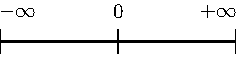
\includegraphics{figs/ns.pdf}
\end{center}
\caption{Number Axis}
\end{figure}

Each point on this axis represents a number. It may be integer or fractional
number. An integer is a whole number like -1, -2, 0, 5, 7 etc. Floating-point
numbers have fractional parts like 1.234. The important fact to note is that
between any two points there exists infinite numbers. In other words between
any two numbers there exists infinite numbers. For example, between 1.2 and 1.3
there are 1.21, 1.22, 1.23..., 1.29. Moreover between 1.21 and 1.22 there are
1.211, 1.212, 1.213 and so on. It enables us to represent a point on this
axis. The numbers I have written are supposedly in decimal number system. Base
of decimal number system is 10. Why because it consists of 10 distinct symbols
0 through 9. Similarly we can have any other number system. Popular number
systems in computers are binary, octal and hexadecimal not to mention decimal
of course.

A number in a generic number system is given below:
\begin{equation}
(.. c_mb^{m-1} + c_{m-1}b^{m-2}+ ... + c_2b^1 + c1_b^0 + c_{-1}b^{-1} +
... + c_{-m}b^{-m} ) \\ = (... c_mc_{m-1}...c_2c_1.c_{-1}...c_{-m})_b
\end{equation}

All the terms with $c$  are called digits. The leftmost or leading digit is
called \textit{most significant digit} and the rightmost or trailing digit is
called \textit{least significant digit}. The . is called a point which
separates the integral part which is towards its left from the fractional part
which is towards its right. $b$  is known as radix or base of the number
system. Note that all digits will be between $0$ to $b-1$. So in our decimal
system $b$  is 10 therefore we have digits from 0 to 9. In binary number system
it is 2 therefore digits permitted are 0 and 1.

\subsection{Binary Number System}
\label{bns}
As the name suggests binary number system has base of 2. Therefore it has only
two symbols. 0 and 1. This is the most popular system for computers because TTL
NAND and NOR gates which are the most basic logic gates using which other gates
are implemented in processor has only two voltage output levels because of
their operation in cut-off and saturation zones. These terms are better
understood with the help of a book on electronics which is out of scope of this
book. All binary numbers consist of 0 and 1. So the count is like 0, 1, 10, 11,
100, 101, 110, 111, 1000 and so on.

\subsubsection{Conversion of Unsigned Decimals and Binaries}
Consider a decimal number. Let us say 53 then how would be convert it to
binary. The technique is that of division. Please examine following carefully:

\hspace*{2cm}
\begin{Verbatim}[frame=single]
  2 | 53 | 1
  ----------
  2 | 26 | 0
  ----------
  2 | 13 | 1
  ----------
  2 | 6  | 0
  ----------
  2 | 3  | 1
  ----------
    | 1  |
\end{Verbatim}

So the binary is $110101_2$. First we divide 53 by 2 and write the
remainder. Then quotient is 26. We repeat the process for 26 therefore
remainder is 0 and quotient is 13. This we go on repeating till we have 1 as
quotient. Note that all the remainders will be 0 or 1 because divisor is
2. Similarly, final quotient is always 1. Now we take final quotient and start
writing remainders from top to bottom.

To convert binary to decimal let us examine following:

$1*2^5 +1*2^4 +0*2^3 +1*2^2 +0*2^1 +1*2^0 =53_{10}$

The power is to 2 because 2 is the base of source. It starts from 0 for unit's
position and increases to 1 and 2 for ten's and hundred's position and so
on. 1's and 0's are the values of that place. If you note carefully powers of 2
grow like 1, 2, 4, 8, 16, 32, 64, 128 and so on. Any number can be written by
using these powers at most one time. For example consider 100. I know it is
less than 128 so I will use 64. Then 36 remains. So I will use 32 and then
4. This means 100=64+32+4  which means power 6, 5 and 2 have been
used. Therefore, I can quickly write down number as $1100100_2$.

\label{fractional binary numbers}
Fractional numbers are slightly more complicated. Let us consider $1.1_2$  . In
decimal it will be $1+\frac{1}{2}$. This is 1.5 in decimal. Note that when you
convert a fractional part of binary to decimal denominator will always be power
of 2. For that matter when you convert from any base to decimal denominator
will be powers of that base. \textbf{Important:} Therefore, when you convert
from decimal to some base n then denominator of that decimal number can have
only those prime factors which are available in the set of prime factors of
$n$.

Let us say we have a fractional number in decimal .59 then to convert it to
decimal we multiply it with 2 which yields 1.018 which is greater than 1 so our
equivalent binary number is .1. Now we subtract 1 from 1.18 to get .18 which
is less than 1 so we multiply it with 2 again to get .36. Now since this is
less than 1 our equivalent binary number is .10. Repeating the process we get
.72 and .100 then 1.44 and .1001. We put 1 in binary part because decimal part
has become greater than 1. Now again we subtract 1 from decimal part to get .44
and repeat the process.

Operations such as addition, subtraction, multiplication and division are
similar in all number systems.

\subsection{2's Complement and 1's Complement}
2's complement and 1's complement are used to convert binary numbers to decimal
values. In 1's complement the number is obtained by inverting bits i.e. making
0 bit to 1 bit and 1 bit to 0 bit of the binary number in question.

Consider the following table which contains some numbers for 1's complement
of some 8-bit numbers.

The 2's complement of an $N$-bit number is defined as the complement with
respect to $2^N$; i.e. it is the result of subtracting the number
from $2^N$, which in binary is one followed by $N$ zeroes. This is also
equivalent to taking the 1's complement and then adding one, since the sum of
a number and its 1's complement is all 1 bits.



%\begin{table}[!bp]
 \begin{center}
\begin{longtable}{|c|r|r|}
\hline
\textbf{Bits}&\textbf{Unsigned Value}&\textbf{1's Complement Value}\\
\hline
0111 1111&127&127\\
\hline
0111 1110&126&126\\
\hline
0000 0010&2&2\\
\hline
0000 0001&1&1\\
\hline
0000 0000&0&0\\
\hline
1111 1111&255&-0\\
\hline
1111 1110&254&-1\\
\hline
1000 0010&130&-125\\
\hline
1000 0001&129&-126\\
\hline
1000 0000&128&-127\\
\hline
 \caption{8-bit 1's complement integers}
\end{longtable}
\end{center}
%\end{table}

For signed numbers MSB(most significant bit) decides sign in both 1's
complement as well as 2's complement. 1's complement has two zeroes. Positive
and negative. As you see in table that 1111 1111 is -0 because MSB is 1 so it
is a negative number and then if you invert all remaining bits then it turns
out to be 0. In a 1's complement system negative numbers are represented by the
arithmetic negative of the value. An $N$-bit 1's complement number system can
represent integers in the range $-2^{N-1} - 1$ to $-2^{N-1} - 1$.

Now it is easy to do addition, subtraction, multiplication, division and other
arithmetic operations. Subtraction for 1's complement is a bit
different. Consider the following:

\begin{Verbatim}[frame=single]
  0000 0110       6
- 0001 0011      19
  ===========   ====
1 1111 0011     -12    -An end-around borrow is produced, and the sign bit
                        of the intermediate result is 1.
- 0000 0001       1    -Subtract the end-around borrow from the result.
  ===========   ====
  1111 0010     -13    -The correct result (6 - 19 = -13)
\end{Verbatim}

Borrows are propagated to the left. If the borrow extends past the end then it
is said to have ``wrapped around'', a condition called an ``end-around
borrow''. When this occurs, the bit must be subtracted from the right-most bit
or least significant bit(LSB). This does not occur in 2's complement arithmetic.

As you see in table and also you can verify the value becomes negative if its
1's complement is computed. However, 2's complement is used on most of
computers because of two zeroes in 1's complement, borrowing being complicated
etc. 

Consider following table of 2's complement 3-bit binary numbers:

%\begin{table}[H]
  \begin{center}
    \begin{longtable}{|c|r|r|}
      \hline
      \textbf{Bits}&\textbf{Unsigned value}&\textbf{2's complement value}\\
      \hline
      011&3&3\\
      \hline
      010&2&2\\
      \hline
      001&1&1\\
      \hline
      000&0&0\\
      \hline
      111&7&-1\\
      \hline
      110&6&-2\\
      \hline
      101&5&-3\\
      \hline
      100&4&-4\\
      \hline
    \caption{3-bit 2's complement integers}
    \end{longtable}
  \end{center}
%\end{table}
Clearly, since $N$-bit 1's complement can represent numbers in range
$-2^{N-1}-1$ to $2^{N-1} + 1$ 2's complement of $N$-bit can represent
$-2^{N-1}$ to $2^{N-1} - 1$ as it does not have negative 0 i.e. its range is
more by 1 number.

The 2' complement system has the advantage that operations of addition,
subtraction, and multiplication are same as unsigned binary numbers (as long as
the inputs are represented in the same number of bits and any overflow beyond
those bits is discarded from the result). This property makes the system both
simpler to implement and capable of easily handling higher precision
arithmetic. Also, as mentioned above zero has only a single 
representation, avoiding the subtleties associated with negative zero, which
exists in 1's complement systems.

The value $v$ of an $N$-bit integer $b_{N-1} b_{N-2} \dots b_0 $is given by the
following formula:

\begin{equation}
v=-b_{N-1} 2^{N-1} + \sum_{i=0}^{N-2} b_i 2^i
\end{equation}

I will leave it up to you, the reader, to perform basic operations like
addition, subtraction, multiplication, division etc.

\section{Compiling and Executing}
\index{program!compilation}
\index{program!execution}
To compile and execute a program create a new file, edit it and save it. The
extension of file should be \texttt{*.c}. For example,
\texttt{myprogram.c}. After that you can give this command at terminal. Here is
the corrected code.

\begin{minted}[frame=single]{c}
#include <stdio.h>

int main()
{
  return 0;
}
\end{minted}

Execute the following command on your command prompt:
\\\\\$gcc nothing.c -o nothing\\\\
Here \texttt{nothing.c} is the name of the file with which it was saved.

Then you will see a file named my program is created by compiler if no errors
were there in your program. In case of errors, like we had in one shown to you
they have to be resolved first. Executable \texttt{nothing} is produced then
you can execute it like
\\\\\$./nothing\\\\
Note that in both the commands \texttt{\$} is not part of command but it is
prompt. For you it may be \texttt{\%} or \texttt{\#} or something fancier
(depends on the imagination of your system administrator). To execute this
command your working directory must be same as the directory your program is
in.

\color{nicered}
\dangersign[3ex] Also, note that on some systems \texttt{TAB} auto completes filename so do
not do the following by accident:
\\\\\$gcc nothing.c -o nothing.c\\\\
\color{black}
This will overwrite your \texttt{nothing.c} by the result of compilation binary
with the same name \texttt{nothing.c}. Let us see how to compile this program
using a Makefile. Edit your \texttt{Makefile} like this:

\begin{minted}[frame=single]{makefile}
#sample Makefile
check-syntax:
    gcc -o nul -Wall -S $(CHK_SOURCES)

nothing: nothing.c
    gcc -Wall -std=c11 -pedantic nothing.c -o nothing
\end{minted}

Now from do this from menu. \texttt{Tools->compile} As the command issue
\texttt{make -k test}. Another way to do the same using keyboard only is type
\texttt{M-x compile} and repeat \texttt{make -k test} as previous time. Your
code will be compiled. Makefiles are better than executing commands 
repeatedly again and again however you must know underlying commands. I will
discuss the compiler options as appropriate. \texttt{-Wall} will enable all the
warnings from \texttt{gcc}, \texttt{-std=c11} enables new features of C11
standard and \texttt{-pedantic} ensures specification conformance. 

So let us get started with basics of C.

\chapter{Basics of C}
There are certain rules in every language, certain grammar which dictates the
way language will be spoken and written. It has a script to write
using. Similarly, programming languages have BNF (Backus-Naur Form)
context-free grammar. There are valid characters in a programming language and
a set of keywords. There are constructs to handle control flow, loops
etc. There are facilities provided by language to deal with numbers and strings
separately, to reuse the code and some basic data structures to facilitate
programming. However, programming language ruleset is very small compared
to a natural programming language. Also, when using natural programming
language like talking to someone or writing something the other person can
understand your intent but in programming you cannot violate rules. The grammar
is context-free. Compilers or interpreters cannot deduce your intent by reading
code. They are not intelligent. You make a mistake and it will refuse to listen
to you no matter what you do. Therefore, it is very essential to understand
these rules very clearly and correctly.

\section{The C Character Set}
The following form the C character set you are allowed to use in it:

\begin{verbatim}
[a-z] [A-Z] [0-9] ~ ! # % ^ & * ( ) - = [ ] \ ; ' , . / _ + { } | : " < > ?
\end{verbatim}
\index{character set}

This means along with other symbols you can use all English alphabets (both
uppercase and lowercase) and Arabic numerals. Symbols like \texttt{\$} and
\texttt{@} are not part of C's character set. But strings can contain any
these characters also. Strings are sequence of characters with double quotes
and double quotes iteself are escaped with \texttt{$\backslash$}. Also,
\texttt{\$} and \texttt{@} can also be value of characters. Characters are
values containing single characters withing single quotes. We will see more of
these in their individual sections. However, English is not the only
spoken language in the world. Therefore in other non-English speaking counties
there are keyboard where certain characters present in above set are not
present. The inventors of C were wise enough to envision this and provide the
facility in form of trigraph sequences. Given below is the trigraph sequence
table:

\begin{table}
 \begin{center}
 \caption{Trigraph Sequences}
\begin{tabular}{|c|c|c|c|c|c|}
\hline
\textbf{Trigraph}&\textbf{Equivalent}&\textbf{Trigraph}&\textbf{Equivalent}&\textbf{Trigraph}&\textbf{Equivalent}\\
\hline
??=&\#&??'&\textasciicircum&??!&|\\
\hline
??(&[&??)&]&??$<$&\{\\
\hline
??$>$&\}&??/&\textbackslash&??-&\textasciitilde\\
\hline
\end{tabular}
\end{center}
\end{table}
\index{trigraph sequences}

However, you should refrain from using trigraph sequences for portability 
reasons as suggested by GNU coding standards.

\section{Keywords}
The following are reserved keywords for C programming language which you are not 
allows to use other than what they are meant for:
\index{keywords}
\begin{table}[H]
 \begin{center}
  \caption{Keywords of C}
  \begin{tabular}{l l l l l}
    auto & break & case & char & const\\
    continue & default & do & double & else\\
    enum & extern & float & for & goto\\
    if & inline & int & long & register\\
    restricted & return & short & signed & sizeof\\
    static & struct & switch & typedef  & union\\
    unsigned & void & volatile & while & \_Bool\\
    \_Complex & \_Imaginary & &\\
  \end{tabular}
 \end{center}
\end{table}

These keywords are special in C as said and cannot be used for variable names 
or funciton names or otherwise other than in strings and comments.

\section{Identifiers}
The names which we give to our variables are known as identifiers. Something 
with which we identify the variables. As you have already seen what is allowed 
in C's character set but not all are allowed in an identifiers name. Only 
alphabets from English language both lowercase and uppercase, Arabic digits from 
zero to nine and underscore (\_) are allowed in an identifiers name. The rule 
for constructing names is that among the allowed characters it can only begin 
with only English alphabets and underscore. Numbers must not be first character. 
For example, \texttt{x, \_myVar, varX} and \texttt{yourId78} are all valid 
names. However, take care with names starting from underscore as they are mostly 
used by different library authors. Invalid identifier examples are \texttt{9x, 
my\$} and \texttt{your age}. Please read this section carefully and make sure 
understand the rules for naming identifiers. Later at the end of chapter there 
are some simple problems to practice with.

\section{Programming}
Let us revisit our first program and try to understand what it does. Here I am 
giving code once again for quick reference:

\begin{minted}{c}
// My first program
/* Description: This program does nothing.*/

#include <stdio.h>

int main(int argc, char* argv[])
{
  return 0;
}
\end{minted}

You can now issue a command as \texttt{\$gcc nothing.c} where 
\texttt{nothing.c} is the filename by which you saved the source code. Note 
that \texttt{\$} is the prompt not part of command itself. Then you can do an 
ls and you will find that \texttt{a.out} is a file which has been produced by 
clang. Now you can run this program by saying \texttt{\$./a.out} and nothing 
will happen. But if you type \texttt{\$echo \$?} then you will find that 0 is 
printed on screen which is nothing but 0 after \texttt{return} of our program.

As you can see this program does almost nothing but it is fairly complete 
program and we can learn a lot from it about C. Let us try to dissect it line
by line. The first line is a comment. 
Whenever C compiler parses C programs and it encounters \texttt{//} it ignores 
rest of line as code i.e. it does not compile them. This type of single line 
comment were introduced in C99 standard and if your compiler is really old the 
compiler may give you error message about it. The second line is
also comments. Anything between \texttt{/*} and \texttt{*/} is ignored like 
\texttt{//}. However, be careful of something like \texttt{/* some comment */
  more comment */}. Such comments will produce error messages and your program
will fail to compile. The reason for this is when first \texttt{*/} is
encountered by parser or compiler it will complete its token for the comment
and then further portion which we intented to be part of comment will cause
syntax error. 

Comments are very integral part of programming. They are used to describe 
various things. You can write whatever you want. They may also be used to 
generate documentation with tools like doxygen. Typically comments should tell
what the program is doing not how. Sometimes how can be covered, when the logic
is really complex. One should be generous while commenting the code.

The next line is \texttt{\#include <stdio.h>}. \texttt{\#include} is a
preprocessor directive. The preprocessor directive is handled by the C
preprocesor which is handled by C preprocessor which looks in four directories
for include files. The include filename comes after \texttt{\#include} either in
angular brackets or double quotes. The C preprocessor looks for these at four
different places at least out of which one or posiibly two is of interest for
now as we are dealing with angular brackets. Depending on the way your compiler
is installed the file \texttt{stdio.h} may be in \texttt{/usr/include} or
\texttt{/usr/local/include} but then again it may be in a non-standard path
also although possibility of that is very less and then it is controlled by
parameters whose discussion is beyond the scope of book. Let us say
\texttt{stdio.h} is present in either of aforementioned directories then the C
preprocessor will copies the contents and pastes them in source file along the
way putting \texttt{\#line} macros which are used for debugging
purposes. \texttt{\#line} macro is discussed later in the chapter which deals
with macros. You can see the output of C preprocessor by typing \texttt{\$gcc
  -E nothing.c} since it will scroll a lot on you terminal you can use a pager
like \texttt{less} to read it. The \texttt{-E} tells \texttt{gcc} to just allow
preprocessoing and not compile and link the file.

I have recorded a video on basics of compilation which you can see at
\url{http://www.youtube.com/watch?v=ARsoVgknRU0}.

Next line is \texttt{int main(int argc, char* argv[])}. Now this is very special
function. Every complete executable(shared objects or dlls or archive
libraririe do not have main even though they are C programs) C program will
have one main function unless you do assembly hacking. This function is where
the programs start. The first word \texttt{int} is a keyword which shirthand
for integer. This signifies the return type of function. \texttt{main} is the
name of the function. Inside parenthesis you see \texttt{int argc} which tells
how many arguments were passed to program and is short form of argument
count. While \texttt{char* argv[]} is a pointer to array which we will see
later. For now let us just remember that it holds all the arguments to the
program including the program name.

Next is a brace. The scope in C is determined by braces. Something outside any
brace has global scope (we will see these later), something inside first level
of brace has function or local scope. Something inside second or more level of
braces have got that particular block scope. Scope here means that when there
will be a closing brace that particular variable which is valid in that scope
will cease to exist. However, we do not have to worry about that yet as we do
not have any variable. Just note that a corresponding closing brace will be the
end of main function. For every opening brace which starts a scope a closing
brace is mandatory.

Next line is \texttt{return 0;} This means whoever has called \texttt{main()}
will get a 0 as \texttt{return} is returning 0. In this case, receiver is the
shell or operating system 
which has invoked the very program. The semicolon is called the terminator and
used also on Java or C++ for example. The very requirement of semicolon is to
terminate the statement and move on to next statement.

However, the program shown does not do much. Let us write a program which has
some more functionality and we can explore more of C. So here is a program
which takes two integers as input from users and presents their sum as
output. Here is the program:

\begin{minted}{c}
// My second program
// Author: Shiv S. Dayal
// Description: It adds two numbers

#include <stdio.h>

int main()
{
  int x=0, y=0, sum=0;

  printf("Please enter an integer:\n");
  scanf("%d", &x);

  printf("Please enter another integer:\n");
  scanf("%d", &y);

  sum = x + y;

  printf("%d + %d = %d\n", x, y, sum);

  return 0;
}
\end{minted}
and the output is:
\begin{verbatim}
shiv@shiv:~/book/code$ ./addition
Please enter an integer:
7
Please enter another integer:
8
7 + 8 = 15
shiv@shiv:~/book/code$
\end{verbatim}

Note that \texttt{shiv@shiv:~/book/code\$} is the prompt.

Let us discuss new lines one by one. The line \texttt{int x=0, y=0, z=0;} is
declaration and definition or initialization of three ints. \texttt{int}
keyword in C is used to represent integers. Now we have three integers with
there values set to 0. Note that how the variables are separated by commas and
terminated by semicolon(as we saw in last program also). We could have also
written it like this:

\begin{minted}{c}
int x;
int y;
int z;

x = 0;
y = 0;
z = 0;
\end{minted}

or

\begin{minted}{c}
int x, y, z;

x = y = z = 0;
\end{minted}

However, the first method is best and most preferred as it prevents use before
definition. \texttt{int} is a data-type in C. \texttt{x, y,} and \texttt{z} are
called variables of type \texttt{int}. This means that the size of these
variables will be same as \texttt{int}. Note that 
C is a statically typed language and all types have predefined memory
requirements. In cour case, \texttt{int} requires 4 bytes on 32-bit and 64-bit
systems but 2 bytes on 16-bit systems.

Here I have created a video about variables of C which you can see at
\url{http://www.youtube.com/watch?feature=player\_embedded\&v=6whuGZwv2-k} and
you can watch another about \texttt{printf} and \texttt{scanf} at
\url{http://www.youtube.com/watch?feature=player\_embedded\&v=U3jCSTR7Ulo}.

Let us learn a bit about \texttt{printf}. This function is declared in
stdio.h. The prototype of \texttt{printf()} is

\begin{minted}{c}
int printf(const char *restrict format, ...);
\end{minted}

The first argument format is what we have in first two function calls. The
second is a \texttt{...} which means it can take variable number of arguments
known as variable-list. We have seen this in the third call.This means it will
take a string with optional variable no. of arguments. The string is called the
format-string and determines what can be printed with supplied arguments. These
\texttt{...} are used to supply variable no. of arguments. In the first two
\texttt{printf()} statements we just print the format-string so that is
simple. However, in the last one, we have format as \texttt{\%d} which
signifies a decimal integer. The integers printed are in the same order in
which they were supplied.

\texttt{scanf()} is scan function which scans for keyboard input. As by now you
know that \texttt{\%d} is for decimal integer but we have not said \texttt{x}
or \texttt{y}. The reason is \texttt{x} and \texttt{y} are values while
\texttt{\&x} and \texttt{\&y} are the addresses of \texttt{x} and \texttt{y} in
memory. \texttt{scanf()} needs the memory address to which it can write the
contents to. You will see \texttt{\&} operator in action later when we deal
with pointers. Just remember for now that to use a simple variable with
\texttt{scanf()} requires \texttt{\&} before its name.

Till now we have just seen only \texttt{int} data-type but then there are more
data types for other types of numbers, characters and strings. Let us see them
one by one.

\section{Data Types}
What are data types? Why C needs data types? C is a statically typed language
that is every variable has a type associated with it. These types determine
what kind of values these variables can hold and how they will be interpreted.
When everything is a voltage level why not just deal with 0s and 1s? The answer
is simple. You need to abstract and segregate how much is required. For
example, say you are given a sequence of 0s and 1s how much can you work with
them. We as humans are not very versed with 0s and 1s. Also, say we encode
character `A' for 10101 will it be easy for you to see A or numbers. Also,
numbers range from $-\infty$ to $\infty$. Also, since C is statically typed the
sizes of data types have to be known at compile time. There are four types of
data types. Integral, floating-point, arrays and pointers. Here, I will deal
with the two former types and leave latter two for later. The integral types
are \texttt{char, short int, int, long} and \texttt{long long} and
floating-point types are \texttt{float, double} and \texttt{long
  double}. \texttt{signed} and \texttt{unsigned} are sign modifiers which also
modified the range of data types but do not affect their memory
requirements. By default all basic data types are \texttt{signed} in nature and
you must qualify you variables with \texttt{unsigned} if you want that
behavior. \texttt{short} and \texttt{long} are modifiers for size which the
data type occupies but I consider them as different types because memory
requirements are different. The ranges of integral data types directly reflect
their memory requirements and if you know how much memory they are going to
occupy you can easily compute their ranges. The range of floating-point comes
from IEEE specification. IEEE standard document 754 governs the binary
representation of floating point numbers which you can read at
\url{http://www.eecs.berkeley.edu/~wkahan/ieee754status/IEEE754.PDF}. This is
not available from IEEE website itself as they sell the specification's
electronic copies.

Let us write a program to find out ranges for integral data types:

\begin{minted}{c}
// Description: It gives ranges of integral data types

#include <stdio.h>
#include <limits.h>

int main()
{
  printf("Size of char is..........%d\n", sizeof(char));
  printf("Size of short int is.....%d\n", sizeof(short int));
  printf("Size of int is...........%d\n", sizeof(int));
  printf("Size of long is..........%d\n", sizeof(long));
  printf("Size of long long is.....%d\n", sizeof(long long));
  printf("Size of float is.........%d\n", sizeof(float));
  printf("Size of double is........%d\n", sizeof(double));
  printf("Size of long double is...%d\n", sizeof(long double));c

  return 0;
}
\end{minted}

Here \texttt{sizeof} is a compile time operator which computes size of any type
passed to it as an argument. So it is computing sizes of all the data types as
shown in the program. The output is given below:

\begin{verbatim}
Size of char is..........1
Size of short int is.....2
Size of int is...........4
Size of long is..........8
Size of long long is.....8
Size of float is.........4
Size of double is........8
Size of long double is...16
\end{verbatim}

Please note that the output shown is on 64-bit machine and it will be different
on 32-bit machines.
\backmatter
\printindex
\end{document}
